\begin{minipage}{0.115\textwidth}
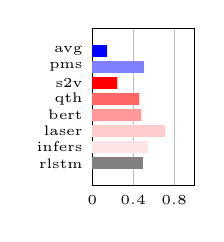
\begin{tikzpicture}

  	\begin{axis}[
    	xbar stacked,
		bar width=4pt,
		enlarge y limits=0.2,
    		symbolic y coords={rlstm,infers,laser,bert,qth,s2v,pms,avg},
		xmin=0,xmax=1,
  		xmajorgrids,
		tickwidth=0pt,
		xtick distance=0.40,
  		ytick=data,
		scale only axis=true,
  		width=1.3cm,height=2cm,
		tick label style={font=\tiny}
  	]

		% avg
  		\addplot[blue,fill] coordinates
  			{(0.140,avg) (0.00,pms) (0.00,s2v) (0.00,qth) (0.00,bert) (0.00,laser) (0.00,infers) (0.00,rlstm)};
		% pms
		\addplot[blue!50,fill] coordinates
			{(0.00,avg) (0.498,pms) (0.00,s2v) (0.00,qth) (0.00,bert) (0.00,laser) (0.00,infers) (0.00,rlstm)};

		% s2v
		\addplot[red,fill] coordinates 
			{(0.00,avg) (0.00,pms) (0.240,s2v) (0.00,qth) (0.00,bert) (0.00,laser) (0.00,infers) (0.00,rlstm)};
		% qth
		\addplot[red!60,fill] coordinates
			{(0.00,avg) (0.00,pms) (0.00,s2v) (0.454,qth) (0.00,bert) (0.00,laser) (0.00,infers) (0.00,rlstm)};
		% bert
		\addplot[red!40,fill] coordinates
			{(0.00,avg) (0.00,pms) (0.00,s2v) (0.00,qth) (0.472,bert) (0.00,laser) (0.00,infers) (0.00,rlstm)};
		% laser
		\addplot[red!20,fill] coordinates
			{(0.00,avg) (0.00,pms) (0.00,s2v) (0.00,qth) (0.00,bert) (0.705,laser) (0.00,infers) (0.00,rlstm)};
		% infersent
		\addplot[red!10,fill] coordinates
			{(0.00,avg) (0.00,pms) (0.00,s2v) (0.00,qth) (0.00,bert) (0.00,laser) (0.537,infers) (0.00,rlstm)};

		% rand lstm
		\addplot[gray,fill] coordinates 
			{(0.00,avg) (0.00,pms) (0.00,s2v) (0.00,qth) (0.00,bert) (0.00,laser) (0.00,infers) (0.487,rlstm)};

  	\end{axis}

\end{tikzpicture}
\end{minipage}
\hfill
\begin{minipage}{0.09\textwidth}
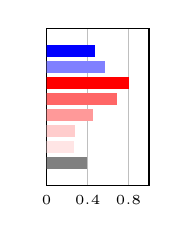
\begin{tikzpicture}

  	\begin{axis}[
    	xbar stacked,
		bar width=4pt,
		enlarge y limits=0.2,
    		symbolic y coords={rlstm,infers,laser,bert,qth,s2v,pms,avg},
		xmin=0,xmax=1,
  		xmajorgrids,
		tickwidth=0pt,
		xtick distance=0.40,
  		ytick=data,
		yticklabels={,,},
		scale only axis=true,
  		width=1.3cm,height=2cm,
		tick label style={font=\tiny}
  	]

		% avg
  		\addplot[blue,fill] coordinates
  			{(0.466,avg) (0.00,pms) (0.00,s2v) (0.00,qth) (0.00,bert) (0.00,laser) (0.00,infers) (0.00,rlstm)};
		% pms
		\addplot[blue!50,fill] coordinates
			{(0.00,avg) (0.564,pms) (0.00,s2v) (0.00,qth) (0.00,bert) (0.00,laser) (0.00,infers) (0.00,rlstm)};

		% s2v
		\addplot[red,fill] coordinates 
			{(0.00,avg) (0.00,pms) (0.799,s2v) (0.00,qth) (0.00,bert) (0.00,laser) (0.00,infers) (0.00,rlstm)};
		% qth
		\addplot[red!60,fill] coordinates
			{(0.00,avg) (0.00,pms) (0.00,s2v) (0.679,qth) (0.00,bert) (0.00,laser) (0.00,infers) (0.00,rlstm)};
		% bert
		\addplot[red!40,fill] coordinates
			{(0.00,avg) (0.00,pms) (0.00,s2v) (0.00,qth) (0.446,bert) (0.00,laser) (0.00,infers) (0.00,rlstm)};
		% laser
		\addplot[red!20,fill] coordinates
			{(0.00,avg) (0.00,pms) (0.00,s2v) (0.00,qth) (0.00,bert) (0.270,laser) (0.00,infers) (0.00,rlstm)};
		% infersent
		\addplot[red!10,fill] coordinates
			{(0.00,avg) (0.00,pms) (0.00,s2v) (0.00,qth) (0.00,bert) (0.00,laser) (0.262,infers) (0.00,rlstm)};

		% rand lstm
		\addplot[gray,fill] coordinates 
			{(0.00,avg) (0.00,pms) (0.00,s2v) (0.00,qth) (0.00,bert) (0.00,laser) (0.00,infers) (0.384,rlstm)};

  	\end{axis}

\end{tikzpicture}
\end{minipage}
\hfill
\begin{minipage}{0.09\textwidth}
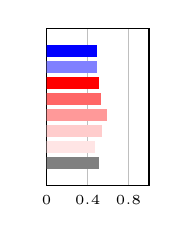
\begin{tikzpicture}

  	\begin{axis}[
    		xbar stacked,
		bar width=4pt,
		enlarge y limits=0.2,
    		symbolic y coords={rlstm,infers,laser,bert,qth,s2v,pms,avg},
		xmin=0,xmax=1,
  		xmajorgrids,
		tickwidth=0pt,
		xtick distance=0.40,
  		ytick=data,
		yticklabels={,,},
		scale only axis=true,
  		width=1.3cm,height=2cm,
		tick label style={font=\tiny}
  	]

		% avg
  		\addplot[blue,fill] coordinates
  			{(0.484,avg) (0.00,pms) (0.00,s2v) (0.00,qth) (0.00,bert) (0.00,laser) (0.00,infers) (0.00,rlstm)};
		% pms
		\addplot[blue!50,fill] coordinates
			{(0.00,avg) (0.487,pms) (0.00,s2v) (0.00,qth) (0.00,bert) (0.00,laser) (0.00,infers) (0.00,rlstm)};

		% s2v
		\addplot[red,fill] coordinates 
			{(0.00,avg) (0.00,pms) (0.501,s2v) (0.00,qth) (0.00,bert) (0.00,laser) (0.00,infers) (0.00,rlstm)};
		% qth
		\addplot[red!60,fill] coordinates
			{(0.00,avg) (0.00,pms) (0.00,s2v) (0.528,qth) (0.00,bert) (0.00,laser) (0.00,infers) (0.00,rlstm)};
		% bert
		\addplot[red!40,fill] coordinates
			{(0.00,avg) (0.00,pms) (0.00,s2v) (0.00,qth) (0.586,bert) (0.00,laser) (0.00,infers) (0.00,rlstm)};
		% laser
		\addplot[red!20,fill] coordinates
			{(0.00,avg) (0.00,pms) (0.00,s2v) (0.00,qth) (0.00,bert) (0.533,laser) (0.00,infers) (0.00,rlstm)};
		% infersent
		\addplot[red!10,fill] coordinates
			{(0.00,avg) (0.00,pms) (0.00,s2v) (0.00,qth) (0.00,bert) (0.00,laser) (0.471,infers) (0.00,rlstm)};

		% rand lstm
		\addplot[gray,fill] coordinates 
			{(0.00,avg) (0.00,pms) (0.00,s2v) (0.00,qth) (0.00,bert) (0.00,laser) (0.00,infers) (0.503,rlstm)};

  	\end{axis}

\end{tikzpicture}
\end{minipage}
\hfill
\begin{minipage}{0.09\textwidth}
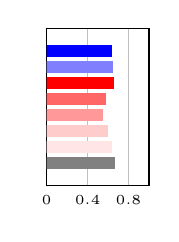
\begin{tikzpicture}

  	\begin{axis}[
   	 	xbar stacked,
		bar width=4pt,
		enlarge y limits=0.2,
    		symbolic y coords={rlstm,infers,laser,bert,qth,s2v,pms,avg},
		xmin=0,xmax=1,
  		xmajorgrids,
		tickwidth=0pt,
		xtick distance=0.40,
  		ytick=data,
		yticklabels={,,},
		scale only axis=true,
  		width=1.3cm,height=2cm,
		tick label style={font=\tiny}
  	]

		% avg
  		\addplot[blue,fill] coordinates
  			{(0.634,avg) (0.00,pms) (0.00,s2v) (0.00,qth) (0.00,bert) (0.00,laser) (0.00,infers) (0.00,rlstm)};
		% pms
		\addplot[blue!50,fill] coordinates
			{(0.00,avg) (0.639,pms) (0.00,s2v) (0.00,qth) (0.00,bert) (0.00,laser) (0.00,infers) (0.00,rlstm)};

		% s2v
		\addplot[red,fill] coordinates 
			{(0.00,avg) (0.00,pms) (0.650,s2v) (0.00,qth) (0.00,bert) (0.00,laser) (0.00,infers) (0.00,rlstm)};
		% qth
		\addplot[red!60,fill] coordinates
			{(0.00,avg) (0.00,pms) (0.00,s2v) (0.579,qth) (0.00,bert) (0.00,laser) (0.00,infers) (0.00,rlstm)};
		% bert
		\addplot[red!40,fill] coordinates
			{(0.00,avg) (0.00,pms) (0.00,s2v) (0.00,qth) (0.549,bert) (0.00,laser) (0.00,infers) (0.00,rlstm)};
		% laser
		\addplot[red!20,fill] coordinates
			{(0.00,avg) (0.00,pms) (0.00,s2v) (0.00,qth) (0.00,bert) (0.590,laser) (0.00,infers) (0.00,rlstm)};
		% infersent
		\addplot[red!10,fill] coordinates
			{(0.00,avg) (0.00,pms) (0.00,s2v) (0.00,qth) (0.00,bert) (0.00,laser) (0.635,infers) (0.00,rlstm)};

		% rand lstm
		\addplot[gray,fill] coordinates 
			{(0.00,avg) (0.00,pms) (0.00,s2v) (0.00,qth) (0.00,bert) (0.00,laser) (0.00,infers) (0.663,rlstm)};

  	\end{axis}

\end{tikzpicture}
\end{minipage}
\hfill
\begin{minipage}{0.09\textwidth}
\begin{center}
\textit{n.\,a.}
\end{center}
\end{minipage}
%\hfill
%\begin{minipage}{0.09\textwidth}
%\begin{tikzpicture}
%
%  	\begin{axis}[
%   	 	xbar stacked,
%		bar width=4pt,
%		enlarge y limits=0.2,
%    		symbolic y coords={rlstm,infers,laser,bert,qth,s2v,pms,avg},
%		xmin=0,xmax=1,
%  		xmajorgrids,
%		tickwidth=0pt,
%		xtick distance=0.40,
%  		ytick=data,
%		yticklabels={,,},
%		scale only axis=true,
%  		width=1.3cm,height=2cm,
%		tick label style={font=\tiny}
%  	]
%
%		% avg
%  		\addplot[blue,fill] coordinates
%  			{(0.08,avg) (0.00,pms) (0.00,s2v) (0.00,qth) (0.00,bert) (0.00,laser) (0.00,infers) (0.00,rlstm)};
%		% pms
%		\addplot[blue!50,fill] coordinates
%			{(0.00,avg) (0.16,pms) (0.00,s2v) (0.00,qth) (0.00,bert) (0.00,laser) (0.00,infers) (0.00,rlstm)};
%
%		% s2v
%		\addplot[red,fill] coordinates 
%			{(0.00,avg) (0.00,pms) (0.16,s2v) (0.00,qth) (0.00,bert) (0.00,laser) (0.00,infers) (0.00,rlstm)};
%		% qth
%		\addplot[red!60,fill] coordinates
%			{(0.00,avg) (0.00,pms) (0.00,s2v) (0.16,qth) (0.00,bert) (0.00,laser) (0.00,infers) (0.00,rlstm)};
%		% bert
%		\addplot[red!40,fill] coordinates
%			{(0.00,avg) (0.00,pms) (0.00,s2v) (0.00,qth) (0.17,bert) (0.00,laser) (0.00,infers) (0.00,rlstm)};
%		% laser
%		\addplot[red!20,fill] coordinates
%			{(0.00,avg) (0.00,pms) (0.00,s2v) (0.00,qth) (0.00,bert) (0.08,laser) (0.00,infers) (0.00,rlstm)};
%		% infersent
%		\addplot[red!10,fill] coordinates
%			{(0.00,avg) (0.00,pms) (0.00,s2v) (0.00,qth) (0.00,bert) (0.00,laser) (0.00,infers) (0.00,rlstm)};
%
%		% rand lstm
%		\addplot[gray,fill] coordinates 
%			{(0.00,avg) (0.00,pms) (0.00,s2v) (0.00,qth) (0.00,bert) (0.00,laser) (0.00,infers) (0.05,rlstm)};
%
%  	\end{axis}
%
%\end{tikzpicture}
%\end{minipage}
\hfill
\begin{minipage}{0.09\textwidth}
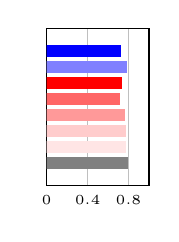
\begin{tikzpicture}

  	\begin{axis}[
    		xbar stacked,
		bar width=4pt,
		enlarge y limits=0.2,
  	  	symbolic y coords={rlstm,infers,laser,bert,qth,s2v,pms,avg},
		xmin=0,xmax=1,
  		xmajorgrids,
		tickwidth=0pt,
		xtick distance=0.40,
  		ytick=data,
		yticklabels={,,},
		scale only axis=true,
  		width=1.3cm,height=2cm,
		tick label style={font=\tiny}
  	]

		% avg
  		\addplot[blue,fill] coordinates
  			{(0.724,avg) (0.00,pms) (0.00,s2v) (0.00,qth) (0.00,bert) (0.00,laser) (0.00,infers) (0.00,rlstm)};
		% pms
		\addplot[blue!50,fill] coordinates
			{(0.00,avg) (0.782,pms) (0.00,s2v) (0.00,qth) (0.00,bert) (0.00,laser) (0.00,infers) (0.00,rlstm)};

		% s2v
		\addplot[red,fill] coordinates 
			{(0.00,avg) (0.00,pms) (0.726,s2v) (0.00,qth) (0.00,bert) (0.00,laser) (0.00,infers) (0.00,rlstm)};
		% qth
		\addplot[red!60,fill] coordinates
			{(0.00,avg) (0.00,pms) (0.00,s2v) (0.707,qth) (0.00,bert) (0.00,laser) (0.00,infers) (0.00,rlstm)};
		% bert
		\addplot[red!40,fill] coordinates
			{(0.00,avg) (0.00,pms) (0.00,s2v) (0.00,qth) (0.761,bert) (0.00,laser) (0.00,infers) (0.00,rlstm)};
		% laser
		\addplot[red!20,fill] coordinates
			{(0.00,avg) (0.00,pms) (0.00,s2v) (0.00,qth) (0.00,bert) (0.765,laser) (0.00,infers) (0.00,rlstm)};
		% infersent
		\addplot[red!10,fill] coordinates
			{(0.00,avg) (0.00,pms) (0.00,s2v) (0.00,qth) (0.00,bert) (0.00,laser) (0.771,infers) (0.00,rlstm)};

		% rand lstm
		\addplot[gray,fill] coordinates 
			{(0.00,avg) (0.00,pms) (0.00,s2v) (0.00,qth) (0.00,bert) (0.00,laser) (0.00,infers) (0.788,rlstm)};

  	\end{axis}

\end{tikzpicture}
\end{minipage}
\hfill
\begin{minipage}{0.09\textwidth}
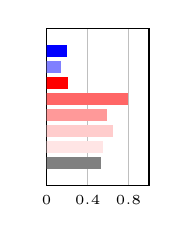
\begin{tikzpicture}

  	\begin{axis}[
   	 	xbar stacked,
		bar width=4pt,
		enlarge y limits=0.2,
   	 	symbolic y coords={rlstm,infers,laser,bert,qth,s2v,pms,avg},
		xmin=0,xmax=1,
  		xmajorgrids,
		tickwidth=0pt,
		xtick distance=0.40,
  		ytick=data,
		yticklabels={,,},
		scale only axis=true,
  		width=1.3cm,height=2cm,
		tick label style={font=\tiny}
  	]

		% avg
  		\addplot[blue,fill] coordinates
  			{(0.195,avg) (0.00,pms) (0.00,s2v) (0.00,qth) (0.00,bert) (0.00,laser) (0.00,infers) (0.00,rlstm)};
		% pms
		\addplot[blue!50,fill] coordinates
			{(0.00,avg) (0.139,pms) (0.00,s2v) (0.00,qth) (0.00,bert) (0.00,laser) (0.00,infers) (0.00,rlstm)};

		% s2v
		\addplot[red,fill] coordinates 
			{(0.00,avg) (0.00,pms) (0.206,s2v) (0.00,qth) (0.00,bert) (0.00,laser) (0.00,infers) (0.00,rlstm)};
		% qth
		\addplot[red!60,fill] coordinates
			{(0.00,avg) (0.00,pms) (0.00,s2v) (0.787,qth) (0.00,bert) (0.00,laser) (0.00,infers) (0.00,rlstm)};
		% bert
		\addplot[red!40,fill] coordinates
			{(0.00,avg) (0.00,pms) (0.00,s2v) (0.00,qth) (0.584,bert) (0.00,laser) (0.00,infers) (0.00,rlstm)};
		% laser
		\addplot[red!20,fill] coordinates
			{(0.00,avg) (0.00,pms) (0.00,s2v) (0.00,qth) (0.00,bert) (0.640,laser) (0.00,infers) (0.00,rlstm)};
		% infersent
		\addplot[red!10,fill] coordinates
			{(0.00,avg) (0.00,pms) (0.00,s2v) (0.00,qth) (0.00,bert) (0.00,laser) (0.543,infers) (0.00,rlstm)};

		% rand lstm
		\addplot[gray,fill] coordinates 
			{(0.00,avg) (0.00,pms) (0.00,s2v) (0.00,qth) (0.00,bert) (0.00,laser) (0.00,infers) (0.525,rlstm)};

  	\end{axis}

\end{tikzpicture}
\end{minipage}
\hfill
\begin{minipage}{0.09\textwidth}
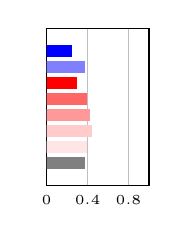
\begin{tikzpicture}

  	\begin{axis}[
   	 	xbar stacked,
		bar width=4pt,
		enlarge y limits=0.2,
    		symbolic y coords={rlstm,infers,laser,bert,qth,s2v,pms,avg},
		xmin=0,xmax=1,
  		xmajorgrids,
		tickwidth=0pt,
		xtick distance=0.40,
  		ytick=data,
		yticklabels={,,},
		scale only axis=true,
  		width=1.3cm,height=2cm,
		tick label style={font=\tiny}
  	]

		% avg
  		\addplot[blue,fill] coordinates
  			{(0.241,avg) (0.00,pms) (0.00,s2v) (0.00,qth) (0.00,bert) (0.00,laser) (0.00,infers) (0.00,rlstm)};
		% pms
		\addplot[blue!50,fill] coordinates
			{(0.00,avg) (0.366,pms) (0.00,s2v) (0.00,qth) (0.00,bert) (0.00,laser) (0.00,infers) (0.00,rlstm)};

		% s2v
		\addplot[red,fill] coordinates 
			{(0.00,avg) (0.00,pms) (0.294,s2v) (0.00,qth) (0.00,bert) (0.00,laser) (0.00,infers) (0.00,rlstm)};
		% qth
		\addplot[red!60,fill] coordinates
			{(0.00,avg) (0.00,pms) (0.00,s2v) (0.387,qth) (0.00,bert) (0.00,laser) (0.00,infers) (0.00,rlstm)};
		% bert
		\addplot[red!40,fill] coordinates
			{(0.00,avg) (0.00,pms) (0.00,s2v) (0.00,qth) (0.413,bert) (0.00,laser) (0.00,infers) (0.00,rlstm)};
		% laser
		\addplot[red!20,fill] coordinates
			{(0.00,avg) (0.00,pms) (0.00,s2v) (0.00,qth) (0.00,bert) (0.435,laser) (0.00,infers) (0.00,rlstm)};
		% infersent
		\addplot[red!10,fill] coordinates
			{(0.00,avg) (0.00,pms) (0.00,s2v) (0.00,qth) (0.00,bert) (0.00,laser) (0.393,infers) (0.00,rlstm)};

		% rand lstm
		\addplot[gray,fill] coordinates 
			{(0.00,avg) (0.00,pms) (0.00,s2v) (0.00,qth) (0.00,bert) (0.00,laser) (0.00,infers) (0.368,rlstm)};

  	\end{axis}

\end{tikzpicture}
\end{minipage}
\hfill
\begin{minipage}{0.09\textwidth}
\begin{center}
\textit{n.\,a.}
\end{center}
\end{minipage}